% Options for packages loaded elsewhere
\PassOptionsToPackage{unicode}{hyperref}
\PassOptionsToPackage{hyphens}{url}
\documentclass[
]{article}
\usepackage{xcolor}
\usepackage[margin=1in]{geometry}
\usepackage{amsmath,amssymb}
\setcounter{secnumdepth}{-\maxdimen} % remove section numbering
\usepackage{iftex}
\ifPDFTeX
  \usepackage[T1]{fontenc}
  \usepackage[utf8]{inputenc}
  \usepackage{textcomp} % provide euro and other symbols
\else % if luatex or xetex
  \usepackage{unicode-math} % this also loads fontspec
  \defaultfontfeatures{Scale=MatchLowercase}
  \defaultfontfeatures[\rmfamily]{Ligatures=TeX,Scale=1}
\fi
\usepackage{lmodern}
\ifPDFTeX\else
  % xetex/luatex font selection
\fi
% Use upquote if available, for straight quotes in verbatim environments
\IfFileExists{upquote.sty}{\usepackage{upquote}}{}
\IfFileExists{microtype.sty}{% use microtype if available
  \usepackage[]{microtype}
  \UseMicrotypeSet[protrusion]{basicmath} % disable protrusion for tt fonts
}{}
\makeatletter
\@ifundefined{KOMAClassName}{% if non-KOMA class
  \IfFileExists{parskip.sty}{%
    \usepackage{parskip}
  }{% else
    \setlength{\parindent}{0pt}
    \setlength{\parskip}{6pt plus 2pt minus 1pt}}
}{% if KOMA class
  \KOMAoptions{parskip=half}}
\makeatother
\usepackage{color}
\usepackage{fancyvrb}
\newcommand{\VerbBar}{|}
\newcommand{\VERB}{\Verb[commandchars=\\\{\}]}
\DefineVerbatimEnvironment{Highlighting}{Verbatim}{commandchars=\\\{\}}
% Add ',fontsize=\small' for more characters per line
\usepackage{framed}
\definecolor{shadecolor}{RGB}{248,248,248}
\newenvironment{Shaded}{\begin{snugshade}}{\end{snugshade}}
\newcommand{\AlertTok}[1]{\textcolor[rgb]{0.94,0.16,0.16}{#1}}
\newcommand{\AnnotationTok}[1]{\textcolor[rgb]{0.56,0.35,0.01}{\textbf{\textit{#1}}}}
\newcommand{\AttributeTok}[1]{\textcolor[rgb]{0.13,0.29,0.53}{#1}}
\newcommand{\BaseNTok}[1]{\textcolor[rgb]{0.00,0.00,0.81}{#1}}
\newcommand{\BuiltInTok}[1]{#1}
\newcommand{\CharTok}[1]{\textcolor[rgb]{0.31,0.60,0.02}{#1}}
\newcommand{\CommentTok}[1]{\textcolor[rgb]{0.56,0.35,0.01}{\textit{#1}}}
\newcommand{\CommentVarTok}[1]{\textcolor[rgb]{0.56,0.35,0.01}{\textbf{\textit{#1}}}}
\newcommand{\ConstantTok}[1]{\textcolor[rgb]{0.56,0.35,0.01}{#1}}
\newcommand{\ControlFlowTok}[1]{\textcolor[rgb]{0.13,0.29,0.53}{\textbf{#1}}}
\newcommand{\DataTypeTok}[1]{\textcolor[rgb]{0.13,0.29,0.53}{#1}}
\newcommand{\DecValTok}[1]{\textcolor[rgb]{0.00,0.00,0.81}{#1}}
\newcommand{\DocumentationTok}[1]{\textcolor[rgb]{0.56,0.35,0.01}{\textbf{\textit{#1}}}}
\newcommand{\ErrorTok}[1]{\textcolor[rgb]{0.64,0.00,0.00}{\textbf{#1}}}
\newcommand{\ExtensionTok}[1]{#1}
\newcommand{\FloatTok}[1]{\textcolor[rgb]{0.00,0.00,0.81}{#1}}
\newcommand{\FunctionTok}[1]{\textcolor[rgb]{0.13,0.29,0.53}{\textbf{#1}}}
\newcommand{\ImportTok}[1]{#1}
\newcommand{\InformationTok}[1]{\textcolor[rgb]{0.56,0.35,0.01}{\textbf{\textit{#1}}}}
\newcommand{\KeywordTok}[1]{\textcolor[rgb]{0.13,0.29,0.53}{\textbf{#1}}}
\newcommand{\NormalTok}[1]{#1}
\newcommand{\OperatorTok}[1]{\textcolor[rgb]{0.81,0.36,0.00}{\textbf{#1}}}
\newcommand{\OtherTok}[1]{\textcolor[rgb]{0.56,0.35,0.01}{#1}}
\newcommand{\PreprocessorTok}[1]{\textcolor[rgb]{0.56,0.35,0.01}{\textit{#1}}}
\newcommand{\RegionMarkerTok}[1]{#1}
\newcommand{\SpecialCharTok}[1]{\textcolor[rgb]{0.81,0.36,0.00}{\textbf{#1}}}
\newcommand{\SpecialStringTok}[1]{\textcolor[rgb]{0.31,0.60,0.02}{#1}}
\newcommand{\StringTok}[1]{\textcolor[rgb]{0.31,0.60,0.02}{#1}}
\newcommand{\VariableTok}[1]{\textcolor[rgb]{0.00,0.00,0.00}{#1}}
\newcommand{\VerbatimStringTok}[1]{\textcolor[rgb]{0.31,0.60,0.02}{#1}}
\newcommand{\WarningTok}[1]{\textcolor[rgb]{0.56,0.35,0.01}{\textbf{\textit{#1}}}}
\usepackage{longtable,booktabs,array}
\newcounter{none} % for unnumbered tables
\usepackage{calc} % for calculating minipage widths
% Correct order of tables after \paragraph or \subparagraph
\usepackage{etoolbox}
\makeatletter
\patchcmd\longtable{\par}{\if@noskipsec\mbox{}\fi\par}{}{}
\makeatother
% Allow footnotes in longtable head/foot
\IfFileExists{footnotehyper.sty}{\usepackage{footnotehyper}}{\usepackage{footnote}}
\makesavenoteenv{longtable}
\usepackage{graphicx}
\makeatletter
\newsavebox\pandoc@box
\newcommand*\pandocbounded[1]{% scales image to fit in text height/width
  \sbox\pandoc@box{#1}%
  \Gscale@div\@tempa{\textheight}{\dimexpr\ht\pandoc@box+\dp\pandoc@box\relax}%
  \Gscale@div\@tempb{\linewidth}{\wd\pandoc@box}%
  \ifdim\@tempb\p@<\@tempa\p@\let\@tempa\@tempb\fi% select the smaller of both
  \ifdim\@tempa\p@<\p@\scalebox{\@tempa}{\usebox\pandoc@box}%
  \else\usebox{\pandoc@box}%
  \fi%
}
% Set default figure placement to htbp
\def\fps@figure{htbp}
\makeatother
\setlength{\emergencystretch}{3em} % prevent overfull lines
\providecommand{\tightlist}{%
  \setlength{\itemsep}{0pt}\setlength{\parskip}{0pt}}
\usepackage{bookmark}
\IfFileExists{xurl.sty}{\usepackage{xurl}}{} % add URL line breaks if available
\urlstyle{same}
\hypersetup{
  hidelinks,
  pdfcreator={LaTeX via pandoc}}

\author{}
\date{\vspace{-2.5em}}

\begin{document}

\section{Cellular Automata Rule-Space
Report}\label{cellular-automata-rule-space-report}

\subsection{Overview}\label{overview}

This project studies two-dimensional binary cellular automata using
Moore neighborhoods and outer-totalistic \texttt{B/S} rules. A rule is
written as \texttt{B.../S...}: the birth set gives the neighbor counts
that turn a dead cell alive, and the survival set gives the neighbor
counts that keep a live cell alive.

The website implements an interactive simulator for Conway's Game of
Life, HighLife, and arbitrary \texttt{B/S} rules. The recorded
experiments extend the interactive work into a 100-rule rule-space study
and a noise/perturbation sweep.

\subsection{Simulator Implementation}\label{simulator-implementation}

The simulator stores the grid as a flat \texttt{Uint8Array(n\ *\ n)} and
renders it to a \texttt{\textless{}canvas\textgreater{}}. This avoids
creating one DOM element per cell and keeps large grids responsive. The
interface exposes:

\begin{itemize}
\tightlist
\item
  Grid sizes: 50 x 50, 100 x 100, 200 x 200, and 300 x 300.
\item
  Rule controls: checkboxes for each birth count and survival count from
  0 through 8.
\item
  Standard controls: randomize, clear, step, run/pause, density, speed,
  and wrapping.
\item
  A displayed rule string such as \texttt{B3/S23} or \texttt{B36/S23}.
\end{itemize}

The headless studies use the same rule representation but run outside
the browser so many trials can be recorded consistently.

\subsection{Experimental Procedure}\label{experimental-procedure}

\subsubsection{Rule Set}\label{rule-set}

The study used 100 rules:

\begin{itemize}
\tightlist
\item
  Conway's Game of Life: \texttt{B3/S23}
\item
  HighLife: \texttt{B36/S23}
\item
  98 seeded random outer-totalistic rules
\end{itemize}

The random rule set was generated from seed \texttt{202609}, so the same
100 rules can be regenerated by the scripts in the repository.

\subsubsection{Baseline Study}\label{baseline-study}

The first baseline study used:

{\def\LTcaptype{none} % do not increment counter
\begin{longtable}[]{@{}lr@{}}
\toprule\noalign{}
Parameter & Value \\
\midrule\noalign{}
\endhead
\bottomrule\noalign{}
\endlastfoot
Rules & 100 \\
Trials per rule & 10 \\
Steps per trial & 500 \\
Grid size & 100 x 100 \\
Initial live-cell density & 24\% \\
Boundary condition & Wrapped torus \\
Seed & 202609 \\
\end{longtable}
}

Each rule was classified by its distribution over the ten random initial
conditions. The dominant class was the most frequent class among those
trials.

\subsubsection{Large-Grid Study}\label{large-grid-study}

The follow-up study reran the same 100 rules on a 500 x 500 grid:

{\def\LTcaptype{none} % do not increment counter
\begin{longtable}[]{@{}lr@{}}
\toprule\noalign{}
Parameter & Value \\
\midrule\noalign{}
\endhead
\bottomrule\noalign{}
\endlastfoot
Rules & 100 \\
Trials per rule & 1 \\
Steps per trial & 500 \\
Grid size & 500 x 500 \\
Initial live-cell density & 24\% \\
Boundary condition & Wrapped torus \\
Seed & 202609 \\
\end{longtable}
}

This run was used to check whether classifications changed when
finite-size effects were reduced. Because this run used one trial per
rule, it is best interpreted as an exploratory comparison against the
100 x 100, 10-trial baseline.

\subsubsection{Noise and Perturbations}\label{noise-and-perturbations}

For the perturbation experiment, each cell was flipped independently
after every rule update with probability \texttt{p}. The tested values
were:

\texttt{p\ =\ 0,\ 0.001,\ 0.005,\ 0.01,\ 0.02,\ 0.05,\ 0.1,\ 0.2,\ 0.5,\ 1.0}

For a given rule and trial, the same starting grid was reused at every
noise probability. That makes the comparison focus on perturbation
strength rather than on a different random initial condition.

\subsection{Measurements}\label{measurements}

For each simulation, the scripts measured:

\begin{itemize}
\tightlist
\item
  Density: \texttt{rho\_t\ =\ live\ cells\ /\ N\^{}2}
\item
  Activity: \texttt{A\_t\ =\ changed\ cells\ /\ N\^{}2}
\item
  Occupied area: bounding-box area containing all live cells, divided by
  \texttt{N\^{}2}
\item
  State repetition: hash table of whole-grid states, used to detect
  fixed points and periodicity
\item
  Density and area trends: late-window averages minus early-window
  averages
\item
  Center-of-mass shift: movement proxy for possible mobile behavior
\end{itemize}

The early and late windows each cover one fifth of the run, with a
minimum of 20 steps.

\subsection{Classification Procedure}\label{classification-procedure}

Each run was classified with a priority-ordered decision rule:

\begin{enumerate}
\def\labelenumi{\arabic{enumi}.}
\tightlist
\item
  \textbf{Extinct}: no live cells remain.
\item
  \textbf{Frozen}: nonzero live cells remain, but final activity is
  approximately zero, or the repeated state has period 1.
\item
  \textbf{Periodic}: a previous whole-grid hash repeats with period
  greater than 1.
\item
  \textbf{Expanding}: occupied area or density increases strongly, or
  the rule reaches very high-density active behavior.
\item
  \textbf{Disordered}: late activity and late density are both high.
\item
  \textbf{Structured Dynamic}: activity persists, but density or
  occupied area remains lower than the disordered regime.
\item
  \textbf{Bounded Dynamic}: low but nonzero persistent activity without
  meeting the previous criteria.
\end{enumerate}

The implementation thresholds were:

\begin{itemize}
\tightlist
\item
  Frozen if final activity is at most one cell change, or if repeat
  period is 1.
\item
  Expanding if area trend is greater than \texttt{0.12}, density trend
  is greater than \texttt{0.08}, or late density is above \texttt{0.65}
  with late activity above \texttt{0.08}.
\item
  Disordered if late activity is above \texttt{0.12} and late density is
  above \texttt{0.35}.
\item
  Structured Dynamic if late activity is above \texttt{0.01} and either
  late occupied area is below \texttt{0.65} or late density is below
  \texttt{0.35}.
\item
  Mobile tag if center-of-mass shift is above \texttt{0.12}, late
  activity is above \texttt{0.005}, and late occupied area is below
  \texttt{0.65}.
\end{itemize}

Reproductive behavior was not assigned automatically. Detecting
self-reproduction reliably would require pattern-level recognition, so
it should be checked visually for candidate rules rather than inferred
from these aggregate statistics alone.

\subsection{Results}\label{results}

\subsubsection{Baseline Classification}\label{baseline-classification}

\begin{figure}
\centering
\pandocbounded{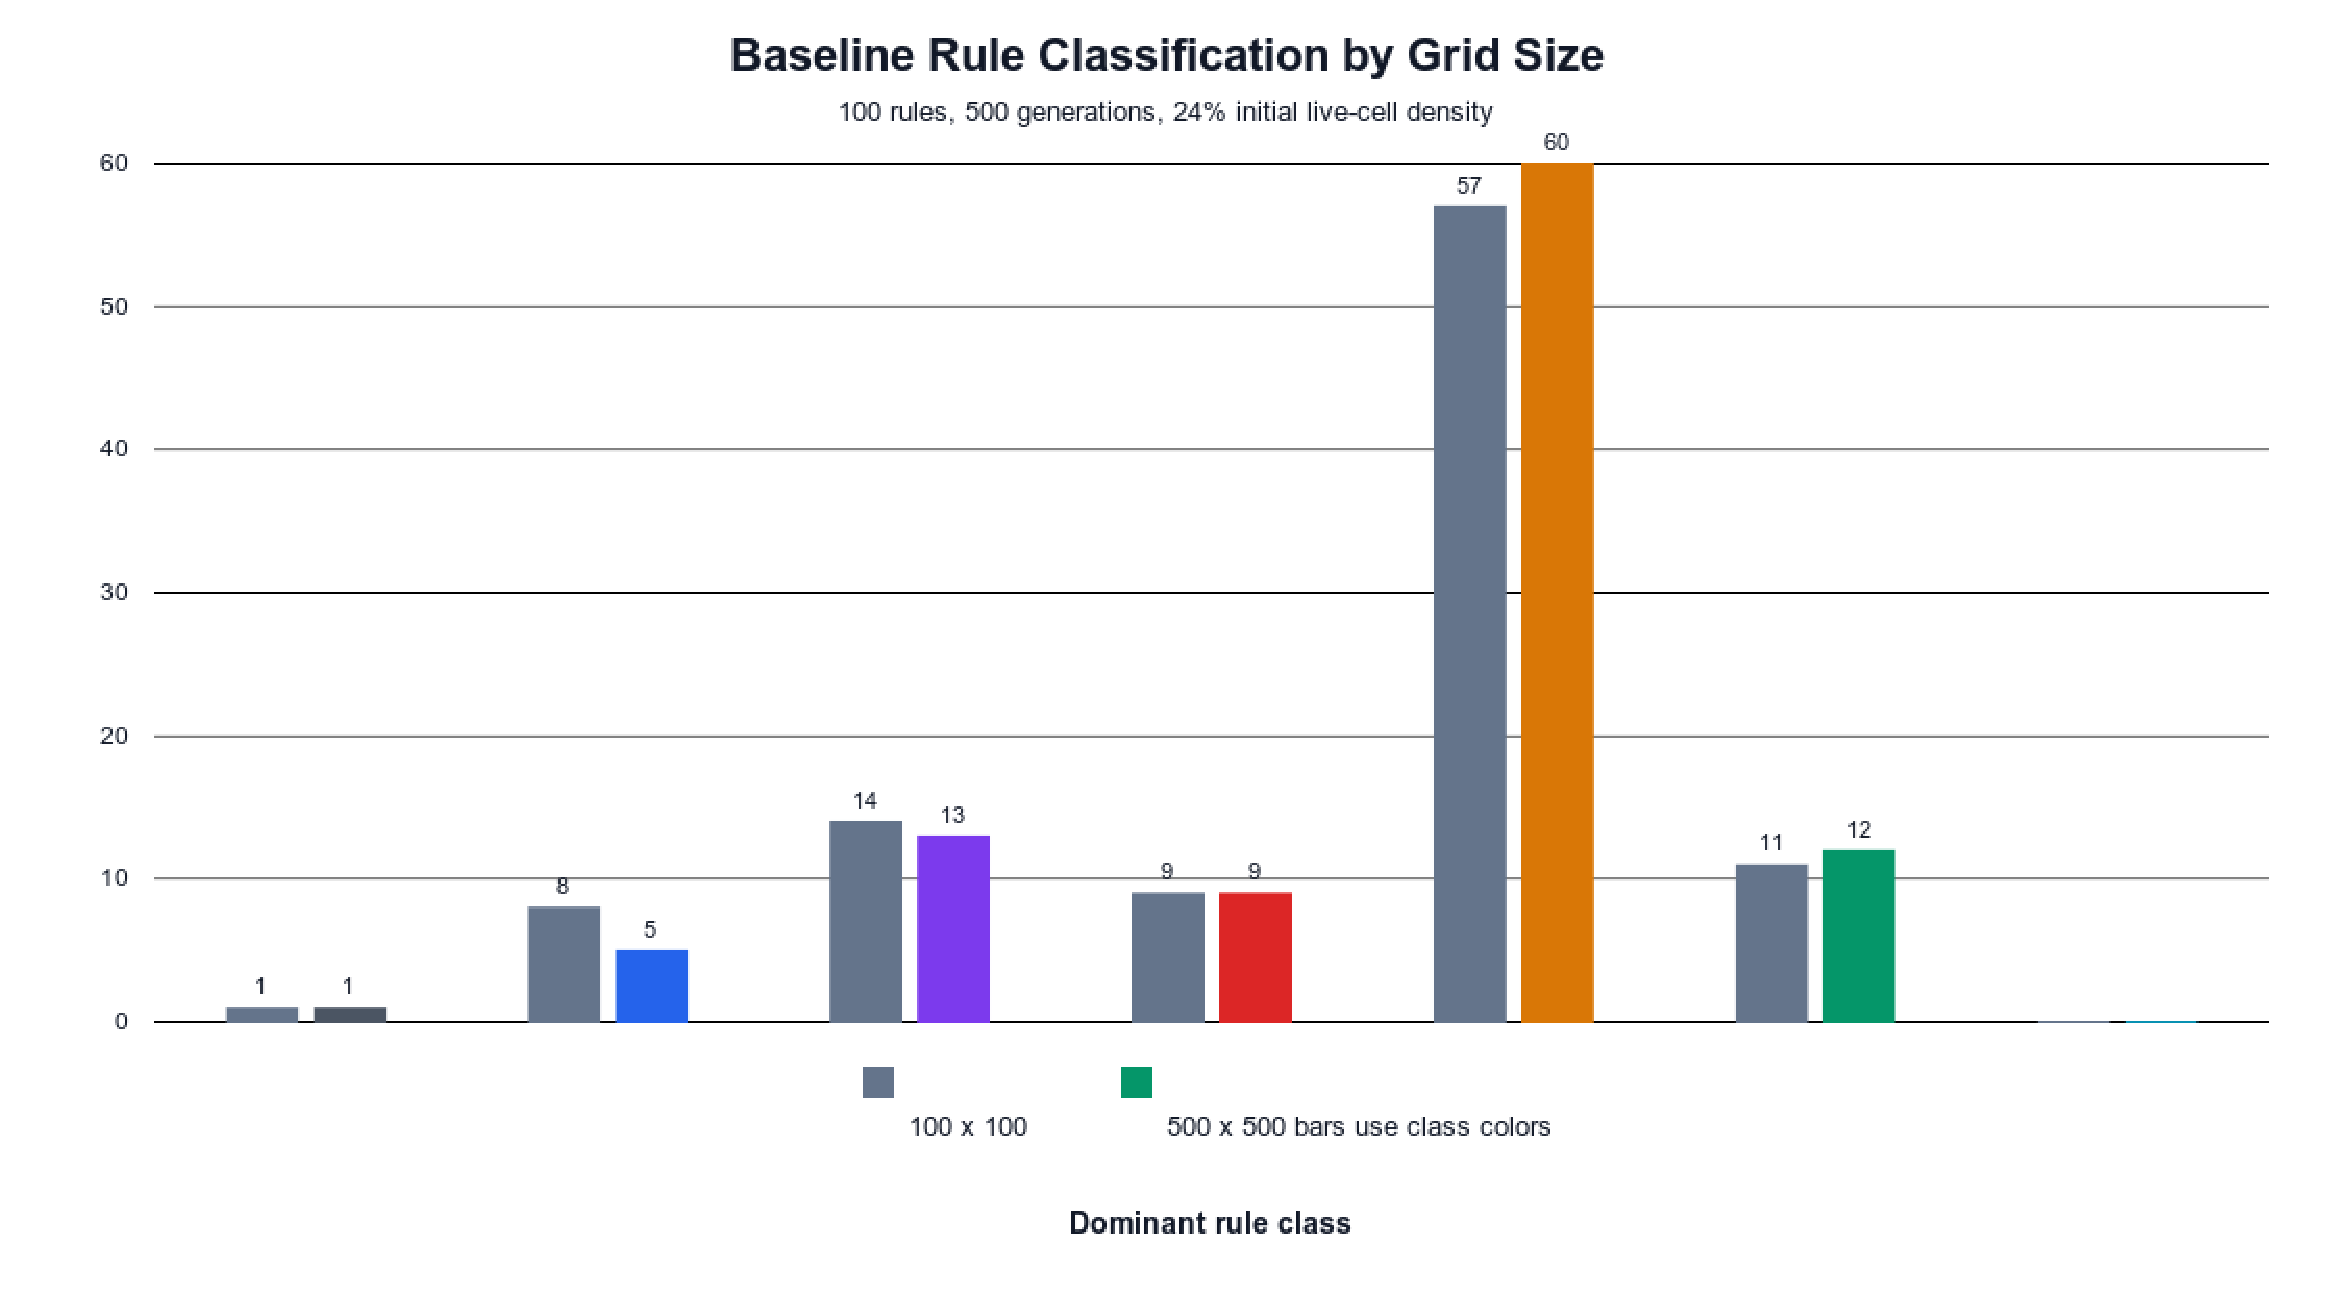
\includegraphics[keepaspectratio]{results/task3_baseline_class_comparison.pdf}}
\caption{Baseline class comparison}
\end{figure}

{\def\LTcaptype{none} % do not increment counter
\begin{longtable}[]{@{}lrr@{}}
\toprule\noalign{}
Class & 100 x 100 rules & 500 x 500 rules \\
\midrule\noalign{}
\endhead
\bottomrule\noalign{}
\endlastfoot
Extinct & 1 & 1 \\
Frozen & 8 & 5 \\
Periodic & 14 & 13 \\
Expanding & 9 & 9 \\
Disordered & 57 & 60 \\
Structured Dynamic & 11 & 12 \\
Bounded Dynamic & 0 & 0 \\
\end{longtable}
}

The overall class distribution was similar at the two grid sizes.
Disordered rules were the largest group in both runs. Increasing the
grid from 100 x 100 to 500 x 500 changed the dominant classification for
7 of the 100 rules:

{\def\LTcaptype{none} % do not increment counter
\begin{longtable}[]{@{}lll@{}}
\toprule\noalign{}
Rule & 100 x 100 class & 500 x 500 class \\
\midrule\noalign{}
\endhead
\bottomrule\noalign{}
\endlastfoot
\texttt{B1578/S035678} & Frozen & Periodic \\
\texttt{B056/S1278} & Periodic & Structured Dynamic \\
\texttt{B234/S2345} & Periodic & Disordered \\
\texttt{B237/S0134567} & Periodic & Disordered \\
\texttt{B2457/S1235678} & Frozen & Periodic \\
\texttt{B17/S2348} & Periodic & Disordered \\
\texttt{B13568/S015678} & Frozen & Periodic \\
\end{longtable}
}

Conway's Life and HighLife both remained \textbf{Structured Dynamic} at
100 x 100 and 500 x 500. At 500 x 500 with no noise, Conway Life had
average final density \texttt{0.054} and average late activity
\texttt{0.036}; HighLife had average final density \texttt{0.044} and
average late activity \texttt{0.032}.

\subsubsection{Noise Sensitivity}\label{noise-sensitivity}

\begin{figure}
\centering
\pandocbounded{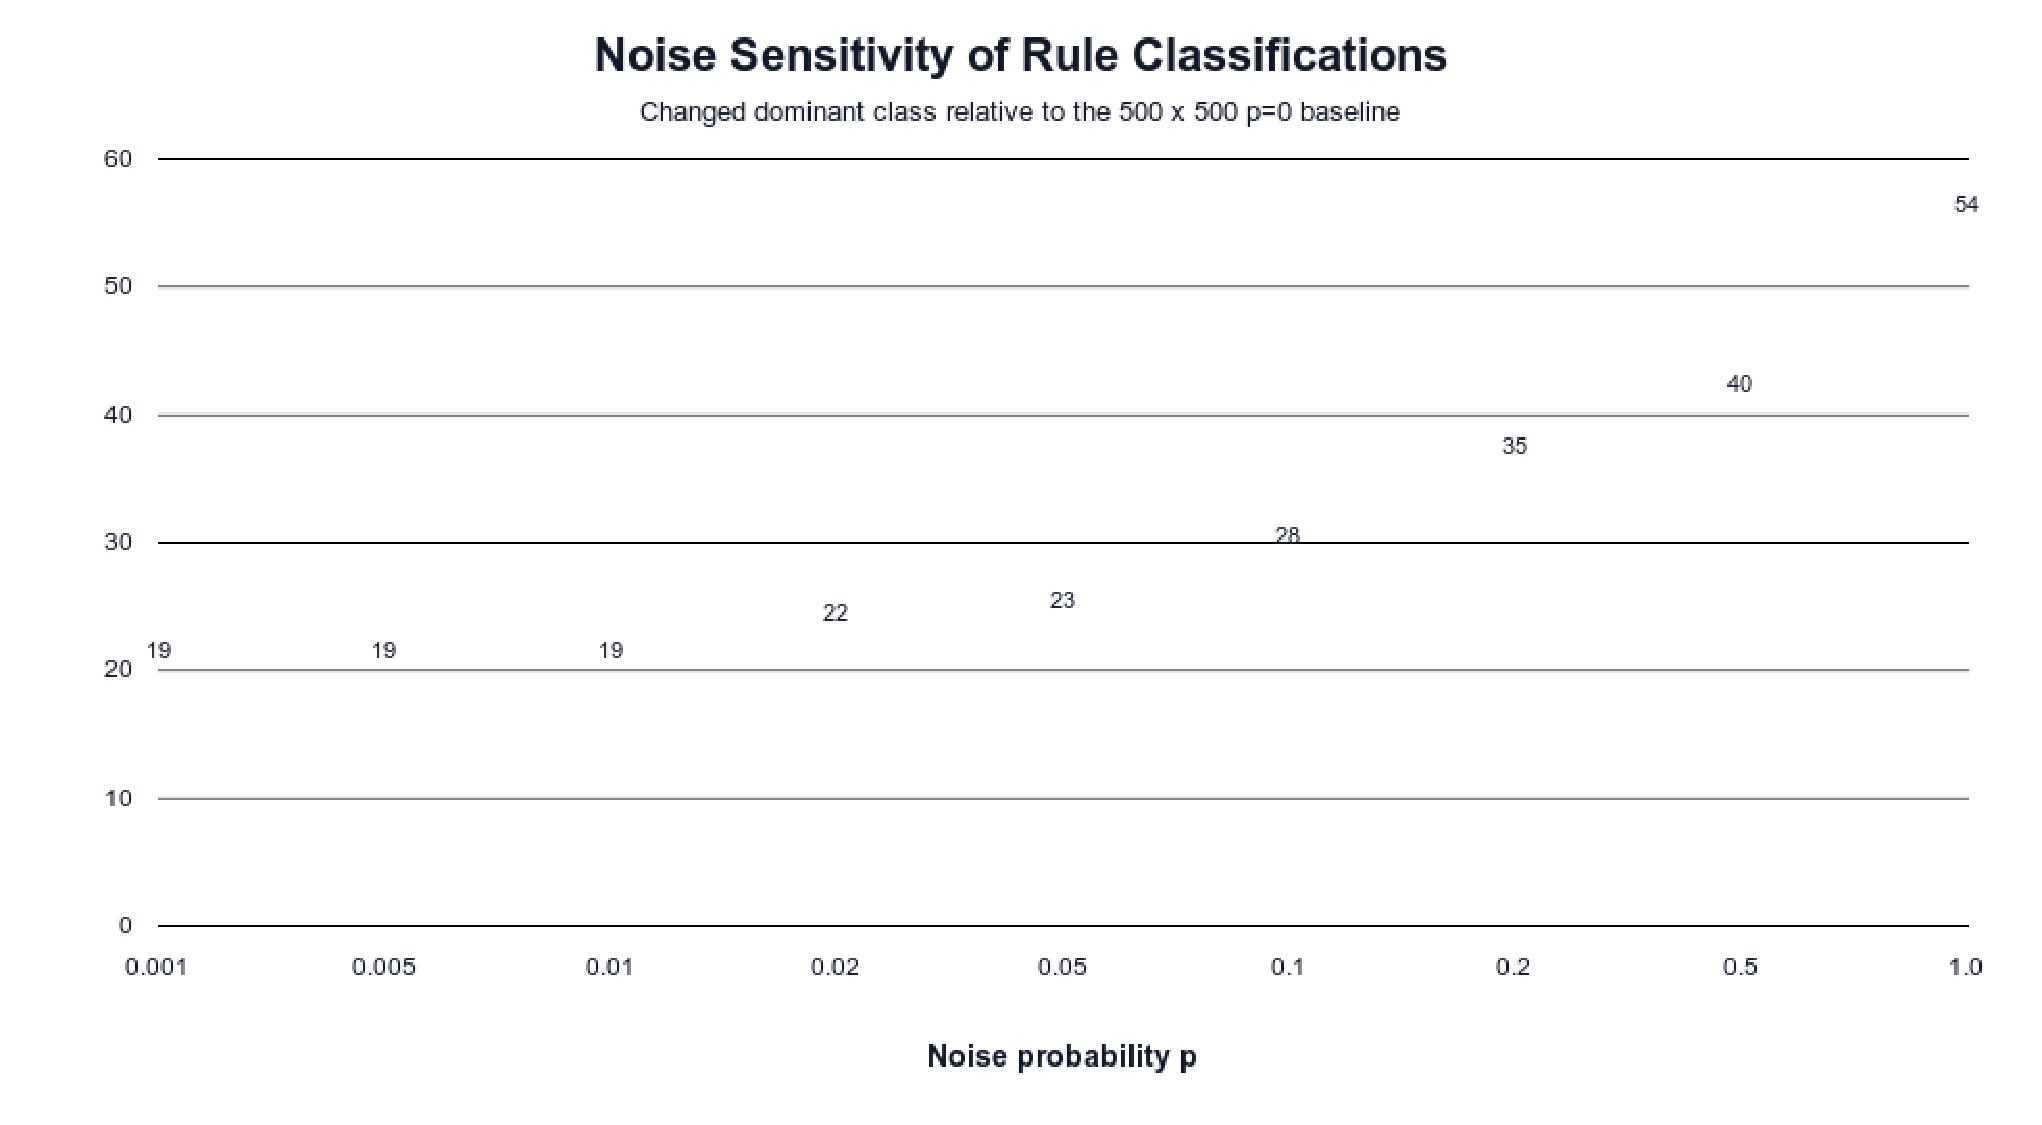
\includegraphics[keepaspectratio]{results/task3_noise_sensitivity.pdf}}
\caption{Rules changed under noise}
\end{figure}

{\def\LTcaptype{none} % do not increment counter
\begin{longtable}[]{@{}lr@{}}
\toprule\noalign{}
Noise probability & Rules whose dominant class changed from
\texttt{p=0} \\
\midrule\noalign{}
\endhead
\bottomrule\noalign{}
\endlastfoot
0.001 & 19 \\
0.005 & 19 \\
0.010 & 19 \\
0.020 & 22 \\
0.050 & 23 \\
0.100 & 28 \\
0.200 & 35 \\
0.500 & 40 \\
1.000 & 54 \\
\end{longtable}
}

Even very small noise changed a noticeable subset of rules. At
\texttt{p=0.001}, 19 rules changed class. Most of these early changes
came from previously Frozen or Periodic rules becoming Bounded Dynamic,
Structured Dynamic, or Disordered. This is expected: a tiny rate of
random flips can prevent exact state repetition, so periodic and frozen
classifications are especially fragile under noise.

At \texttt{p=0.5}, all 100 rules were classified as Disordered. This is
the clearest perturbation result: when every cell has a 50\% chance of
being flipped after each update, the rule dynamics are overwhelmed by
noise and the grid approaches high-activity random behavior.

The \texttt{p=1.0} case is special. It is not random noise in the usual
sense; every cell is flipped after every update. This produces
deterministic complement dynamics, so the classifications spread back
across Frozen, Periodic, Expanding, Disordered, Structured Dynamic, and
Bounded Dynamic rather than remaining all Disordered.

\subsubsection{Class Distribution Across Noise
Values}\label{class-distribution-across-noise-values}

\begin{figure}
\centering
\pandocbounded{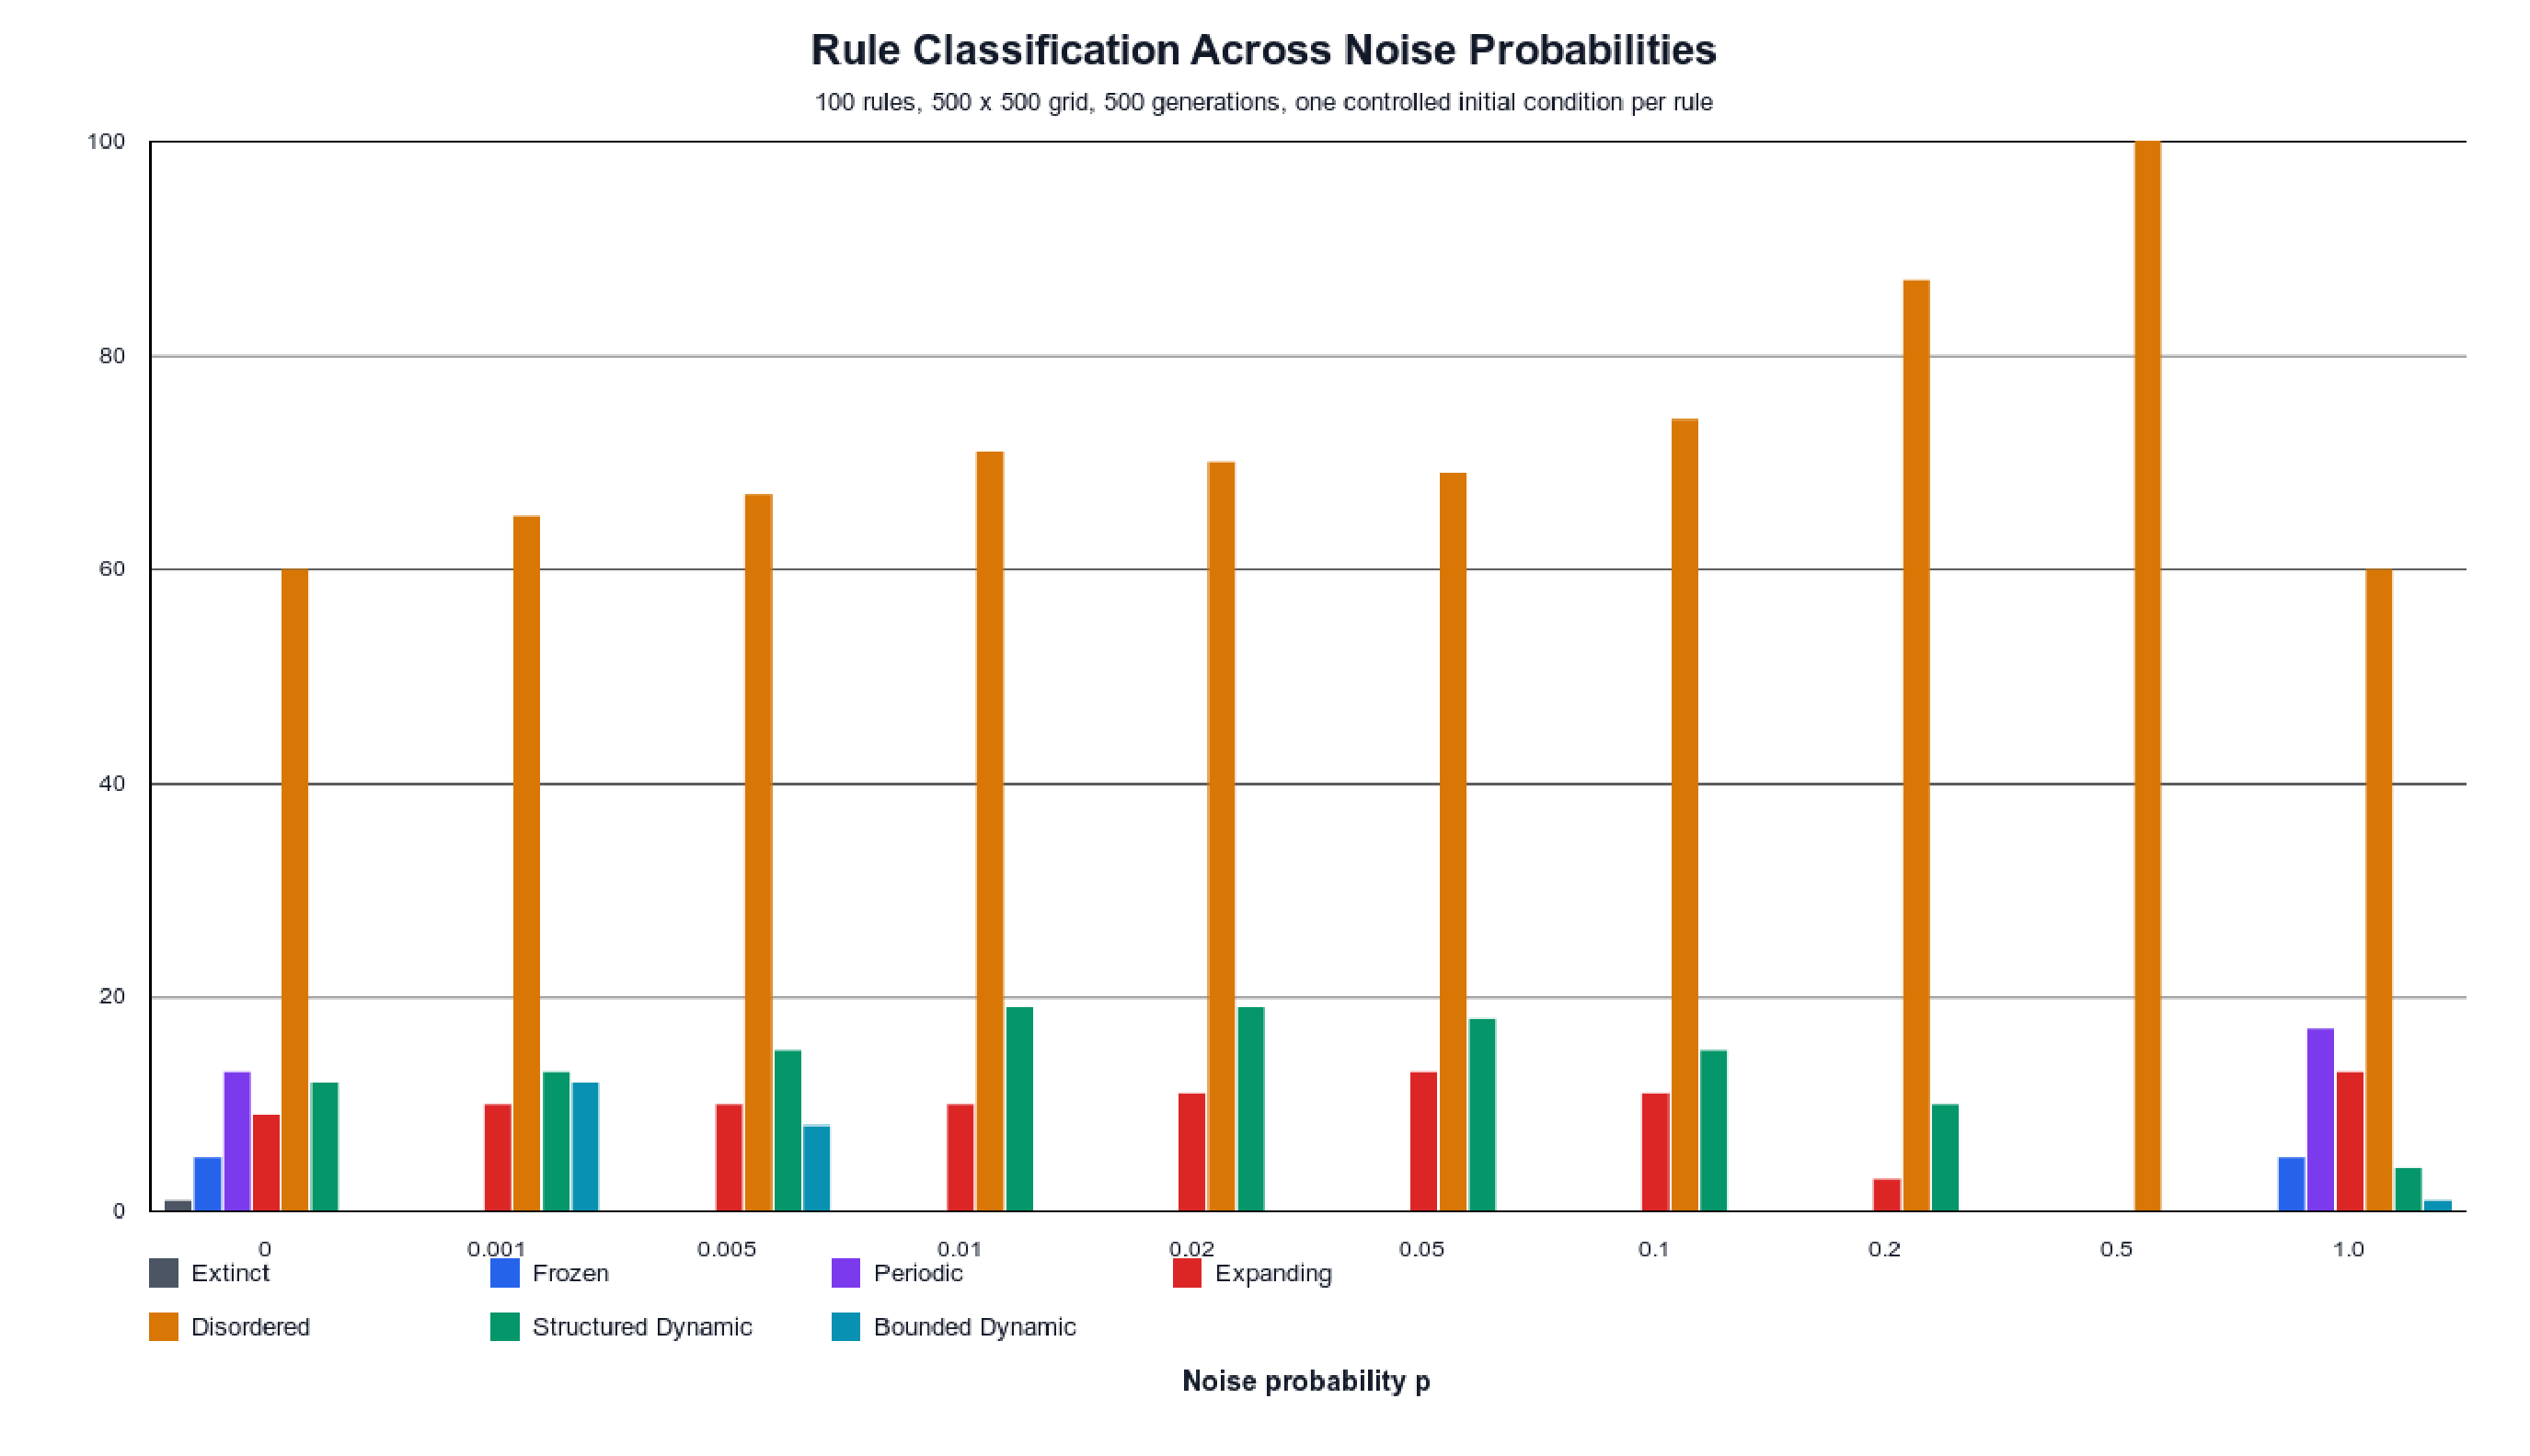
\includegraphics[keepaspectratio]{results/task3_noise_classification_histogram.pdf}}
\caption{Grouped histogram of rule classifications across noise
probabilities}
\end{figure}

{\def\LTcaptype{none} % do not increment counter
\begin{longtable}[]{@{}
  >{\raggedright\arraybackslash}p{(\linewidth - 14\tabcolsep) * \real{0.0968}}
  >{\raggedleft\arraybackslash}p{(\linewidth - 14\tabcolsep) * \real{0.1290}}
  >{\raggedleft\arraybackslash}p{(\linewidth - 14\tabcolsep) * \real{0.1290}}
  >{\raggedleft\arraybackslash}p{(\linewidth - 14\tabcolsep) * \real{0.1290}}
  >{\raggedleft\arraybackslash}p{(\linewidth - 14\tabcolsep) * \real{0.1290}}
  >{\raggedleft\arraybackslash}p{(\linewidth - 14\tabcolsep) * \real{0.1290}}
  >{\raggedleft\arraybackslash}p{(\linewidth - 14\tabcolsep) * \real{0.1290}}
  >{\raggedleft\arraybackslash}p{(\linewidth - 14\tabcolsep) * \real{0.1290}}@{}}
\toprule\noalign{}
\begin{minipage}[b]{\linewidth}\raggedright
Noise
\end{minipage} & \begin{minipage}[b]{\linewidth}\raggedleft
Extinct
\end{minipage} & \begin{minipage}[b]{\linewidth}\raggedleft
Frozen
\end{minipage} & \begin{minipage}[b]{\linewidth}\raggedleft
Periodic
\end{minipage} & \begin{minipage}[b]{\linewidth}\raggedleft
Expanding
\end{minipage} & \begin{minipage}[b]{\linewidth}\raggedleft
Disordered
\end{minipage} & \begin{minipage}[b]{\linewidth}\raggedleft
Structured Dynamic
\end{minipage} & \begin{minipage}[b]{\linewidth}\raggedleft
Bounded Dynamic
\end{minipage} \\
\midrule\noalign{}
\endhead
\bottomrule\noalign{}
\endlastfoot
0.000 & 1 & 5 & 13 & 9 & 60 & 12 & 0 \\
0.001 & 0 & 0 & 0 & 10 & 65 & 13 & 12 \\
0.005 & 0 & 0 & 0 & 10 & 67 & 15 & 8 \\
0.010 & 0 & 0 & 0 & 10 & 71 & 19 & 0 \\
0.020 & 0 & 0 & 0 & 11 & 70 & 19 & 0 \\
0.050 & 0 & 0 & 0 & 13 & 69 & 18 & 0 \\
0.100 & 0 & 0 & 0 & 11 & 74 & 15 & 0 \\
0.200 & 0 & 0 & 0 & 3 & 87 & 10 & 0 \\
0.500 & 0 & 0 & 0 & 0 & 100 & 0 & 0 \\
1.000 & 0 & 5 & 17 & 13 & 60 & 4 & 1 \\
\end{longtable}
}

The grouped histogram shows a sharp loss of exact Extinct, Frozen, and
Periodic outcomes as soon as small stochastic perturbations are
introduced. The middle range of noise shifts the rule set toward
Disordered classifications. Structured Dynamic behavior persists for
some rules through moderate noise, but it declines as \texttt{p}
approaches \texttt{0.5}.

\subsubsection{Conway Life and HighLife Under
Noise}\label{conway-life-and-highlife-under-noise}

{\def\LTcaptype{none} % do not increment counter
\begin{longtable}[]{@{}
  >{\raggedright\arraybackslash}p{(\linewidth - 12\tabcolsep) * \real{0.1200}}
  >{\raggedright\arraybackslash}p{(\linewidth - 12\tabcolsep) * \real{0.1200}}
  >{\raggedleft\arraybackslash}p{(\linewidth - 12\tabcolsep) * \real{0.1600}}
  >{\raggedleft\arraybackslash}p{(\linewidth - 12\tabcolsep) * \real{0.1600}}
  >{\raggedright\arraybackslash}p{(\linewidth - 12\tabcolsep) * \real{0.1200}}
  >{\raggedleft\arraybackslash}p{(\linewidth - 12\tabcolsep) * \real{0.1600}}
  >{\raggedleft\arraybackslash}p{(\linewidth - 12\tabcolsep) * \real{0.1600}}@{}}
\toprule\noalign{}
\begin{minipage}[b]{\linewidth}\raggedright
Noise
\end{minipage} & \begin{minipage}[b]{\linewidth}\raggedright
Conway Life class
\end{minipage} & \begin{minipage}[b]{\linewidth}\raggedleft
Conway density
\end{minipage} & \begin{minipage}[b]{\linewidth}\raggedleft
Conway activity
\end{minipage} & \begin{minipage}[b]{\linewidth}\raggedright
HighLife class
\end{minipage} & \begin{minipage}[b]{\linewidth}\raggedleft
HighLife density
\end{minipage} & \begin{minipage}[b]{\linewidth}\raggedleft
HighLife activity
\end{minipage} \\
\midrule\noalign{}
\endhead
\bottomrule\noalign{}
\endlastfoot
0.000 & Structured Dynamic & 0.054 & 0.036 & Structured Dynamic & 0.044
& 0.032 \\
0.001 & Structured Dynamic & 0.075 & 0.061 & Structured Dynamic & 0.059
& 0.054 \\
0.005 & Structured Dynamic & 0.086 & 0.078 & Structured Dynamic & 0.121
& 0.116 \\
0.010 & Structured Dynamic & 0.136 & 0.129 & Structured Dynamic & 0.194
& 0.194 \\
0.020 & Structured Dynamic & 0.232 & 0.229 & Structured Dynamic & 0.279
& 0.285 \\
0.050 & Structured Dynamic & 0.319 & 0.327 & Structured Dynamic & 0.348
& 0.365 \\
0.100 & Disordered & 0.359 & 0.377 & Disordered & 0.386 & 0.409 \\
0.200 & Disordered & 0.403 & 0.426 & Disordered & 0.420 & 0.451 \\
0.500 & Disordered & 0.499 & 0.500 & Disordered & 0.498 & 0.500 \\
1.000 & Frozen & 1.000 & 0.000 & Periodic & 0.993 & 0.000 \\
\end{longtable}
}

Both Conway Life and HighLife were robustly classified as Structured
Dynamic through \texttt{p=0.05}. At \texttt{p=0.1}, both crossed into
Disordered behavior. The density and activity values show why: the
perturbations raise the live-cell density and changed-cell fraction
until localized structures are no longer the dominant behavior.

\subsection{Interpretation}\label{interpretation}

The main conclusion is that measurement-based classes can separate
several broad regimes: extinction, stability, periodicity, expansion,
disorder, and structured dynamics. However, the boundary between
Structured Dynamic and Disordered is quantitative and
threshold-dependent. Rules near that boundary should be rerun with more
initial conditions and longer simulations before being treated as final
examples.

The 500 x 500 baseline suggests that most classifications are not purely
small-grid artifacts: 93 of 100 rules kept the same dominant class. The
seven changes are still important because they show that Frozen and
Periodic labels can be sensitive to grid size and initial-condition
sampling.

Noise affects exact classifications most strongly for Frozen and
Periodic rules, because random flips disrupt exact rest states and exact
cycle repeats. Conway Life and HighLife are more robust: they remain
Structured Dynamic under low and moderate perturbation, then become
Disordered once noise is large enough to dominate local structure.

\subsection{Interesting Questions}\label{interesting-questions}

\begin{enumerate}
\def\labelenumi{\arabic{enumi}.}
\item
  \textbf{Attractor counting:} How does the number of fixed and
  period-\texttt{k} configurations of a Life-like rule scale with grid
  size, and can they be counted efficiently?
\item
  \textbf{Emergence thresholds:} Given that such structures are
  possible, under what density and spatial-isolation conditions do they
  actually emerge from random initial conditions? Is there a predictable
  finite-size or critical threshold?
\end{enumerate}

\subsection{Limitations}\label{limitations}

\begin{itemize}
\tightlist
\item
  The 100 x 100 baseline used 10 trials per rule, but the 500 x 500
  noise sweep used one trial per rule/probability.
\item
  The classifier uses whole-grid hashes for periodicity, so local
  oscillators inside noisy backgrounds are not counted as Periodic.
\item
  The Mobile tag is only a center-of-mass proxy and did not identify
  reliable mobile or reproductive behavior in the recorded runs.
\item
  Reproduction was not automatically detected.
\item
  Longer runs may change classifications for slow-growing, slowly
  stabilizing, or rare-structure rules.
\end{itemize}

\subsection{Reproducibility}\label{reproducibility}

Run the browser simulator by opening \texttt{index.html}, or serve the
project locally with:

\begin{Shaded}
\begin{Highlighting}[]
\ExtensionTok{python3} \AttributeTok{{-}m}\NormalTok{ http.server 8080}
\end{Highlighting}
\end{Shaded}

Reproduce the 100 x 100 baseline:

\begin{Shaded}
\begin{Highlighting}[]
\ExtensionTok{node}\NormalTok{ scripts/run\_task3\_study.js}
\end{Highlighting}
\end{Shaded}

Reproduce the 500 x 500 baseline and noise sweep:

\begin{Shaded}
\begin{Highlighting}[]
\FunctionTok{clang}\NormalTok{++ }\AttributeTok{{-}std}\OperatorTok{=}\NormalTok{c++17 }\AttributeTok{{-}O3} \AttributeTok{{-}pthread}\NormalTok{ scripts/run\_large\_noise\_study.cpp }\AttributeTok{{-}o}\NormalTok{ /tmp/run\_large\_noise\_study}
\ExtensionTok{/tmp/run\_large\_noise\_study}
\end{Highlighting}
\end{Shaded}

Regenerate report figures:

\begin{Shaded}
\begin{Highlighting}[]
\ExtensionTok{python3}\NormalTok{ scripts/plot\_noise\_classification\_histogram.py}
\ExtensionTok{python3}\NormalTok{ scripts/plot\_report\_figures.py}
\end{Highlighting}
\end{Shaded}

The raw results are stored in \texttt{results/}.

\end{document}
